%! TeX program = lualatex
\documentclass[a4paper]{article} 

% packages
\usepackage{microtype}      % Slightly tweak font spacing for aesthetics
\usepackage[english]{babel} % Language hyphenation and typographical rules
\usepackage{changepage}     % adjust margins on the fly
\usepackage{booktabs}  % For better-looking tables
\usepackage{pgfplotstable}  % For reading and displaying CSV/TSV files

\usepackage[final, colorlinks = true, urlcolor = black, linkcolor = black, citecolor = black]{hyperref} 
\usepackage{fontspec}
% \setmainfont{EB Garamond}
% \setmonofont[Scale=MatchLowercase]{Deja Vu Sans Mono}

\setmainfont{EB Garamond}[
    Ligatures=TeX,
    Numbers=OldStyle
]

% Fallback font (for missing characters)
\setmainfont{EB Garamond}[
    % Ligatures=TeX,
    % Numbers=OldStyle
]

\newfontfamily{\emojifont}{Noto Color Emoji}[Renderer=Harfbuzz]

% Monospace font configuration
\setmonofont[Scale=MatchLowercase]{DejaVu Sans Mono}

\usepackage[backend=biber, style=numeric, date=iso, urldate=iso]{biblatex}
\addbibresource{references.bib}
\DeclareFieldFormat{urldate}{Accessed on: #1}

\usepackage{minted}
\usemintedstyle{algol_nu}
\usepackage{xcolor}

\usepackage{pgfplots}
\pgfplotsset{width=\textwidth,compat=1.9}

\usepackage{caption}
\newenvironment{code}{\captionsetup{type=listing}}{}
\captionsetup[listing]{skip=0pt}
\setlength{\abovecaptionskip}{5pt}
\setlength{\belowcaptionskip}{5pt}

\usepackage[yyyymmdd]{datetime}
\renewcommand{\dateseparator}{--}

\usepackage{titlesec}
% \titleformat{\section}{\LARGE\bfseries}{}{}{}[\titlerule]
% \titleformat{\subsection}{\Large\bfseries}{}{0em}{}
% \titlespacing{\subsection}{0em}{-0.7em}{0em}
%
% \titleformat{\subsubsection}{\large\bfseries}{}{0em}{$\bullet$ }
% \titlespacing{\subsubsection}{1em}{-0.7em}{0em}

% margins
\addtolength{\hoffset}{-2.25cm}
\addtolength{\textwidth}{4.5cm}
\addtolength{\voffset}{-3.25cm}
\addtolength{\textheight}{5cm}
\setlength{\parskip}{0pt}
\setlength{\parindent}{0in}
% \setcounter{secnumdepth}{0}

\begin{document}
\hrule \medskip
\begin{minipage}{0.295\textwidth} 
    \raggedright
    \footnotesize 
    \begin{tabular}{@{}l l}
        Name: & Andrew Hayes \\
        Student ID: & 21321503 \\
        E-mail: & \href{mailto://a.hayes18@universityofgalway.ie}{\texttt{a.hayes18@universityofgalway.ie}} \\
    \end{tabular}
\end{minipage}
\begin{minipage}{0.4\textwidth} 
    \centering 
    \vspace{0.4em}
    \LARGE
    \textsc{ct437} \\ 
\end{minipage}
\begin{minipage}{0.295\textwidth} 
    \raggedleft
    \today
\end{minipage}
\medskip\hrule 
\begin{center}
    \normalsize
    Assignment 2: Using \& Benchmarking Block Ciphers with OpenSSL
\end{center}
\hrule
\medskip

\section{Block Cipher Benchmarking}
\begin{table}[H]
    \centering
    \pgfplotstabletypeset[
        col sep=tab, % Specifies that the file is tab-separated
        string type, % Ensures text columns are treated correctly
        header=true, % Includes the header row
        columns/Cipher/.style={column name=Cipher},
        columns/Key Size/.style={column name=Key Size (bits)},
        columns/Mode/.style={column name=Mode},
        columns/Data Size (MB)/.style={column name=Data Size (MB)},
        columns/Encryption Time (s)/.style={column name=Encryption Time (s)},
        columns/Decryption Time (s)/.style={column name=Decryption Time (s)},
        every head row/.style={before row=\toprule, after row=\midrule},
        every last row/.style={after row=\bottomrule}
    ] {../code/results.tsv} % Filename
    \caption{Benchmarking results from TSV file}
\end{table}

\begin{figure}[H]
    \centering
    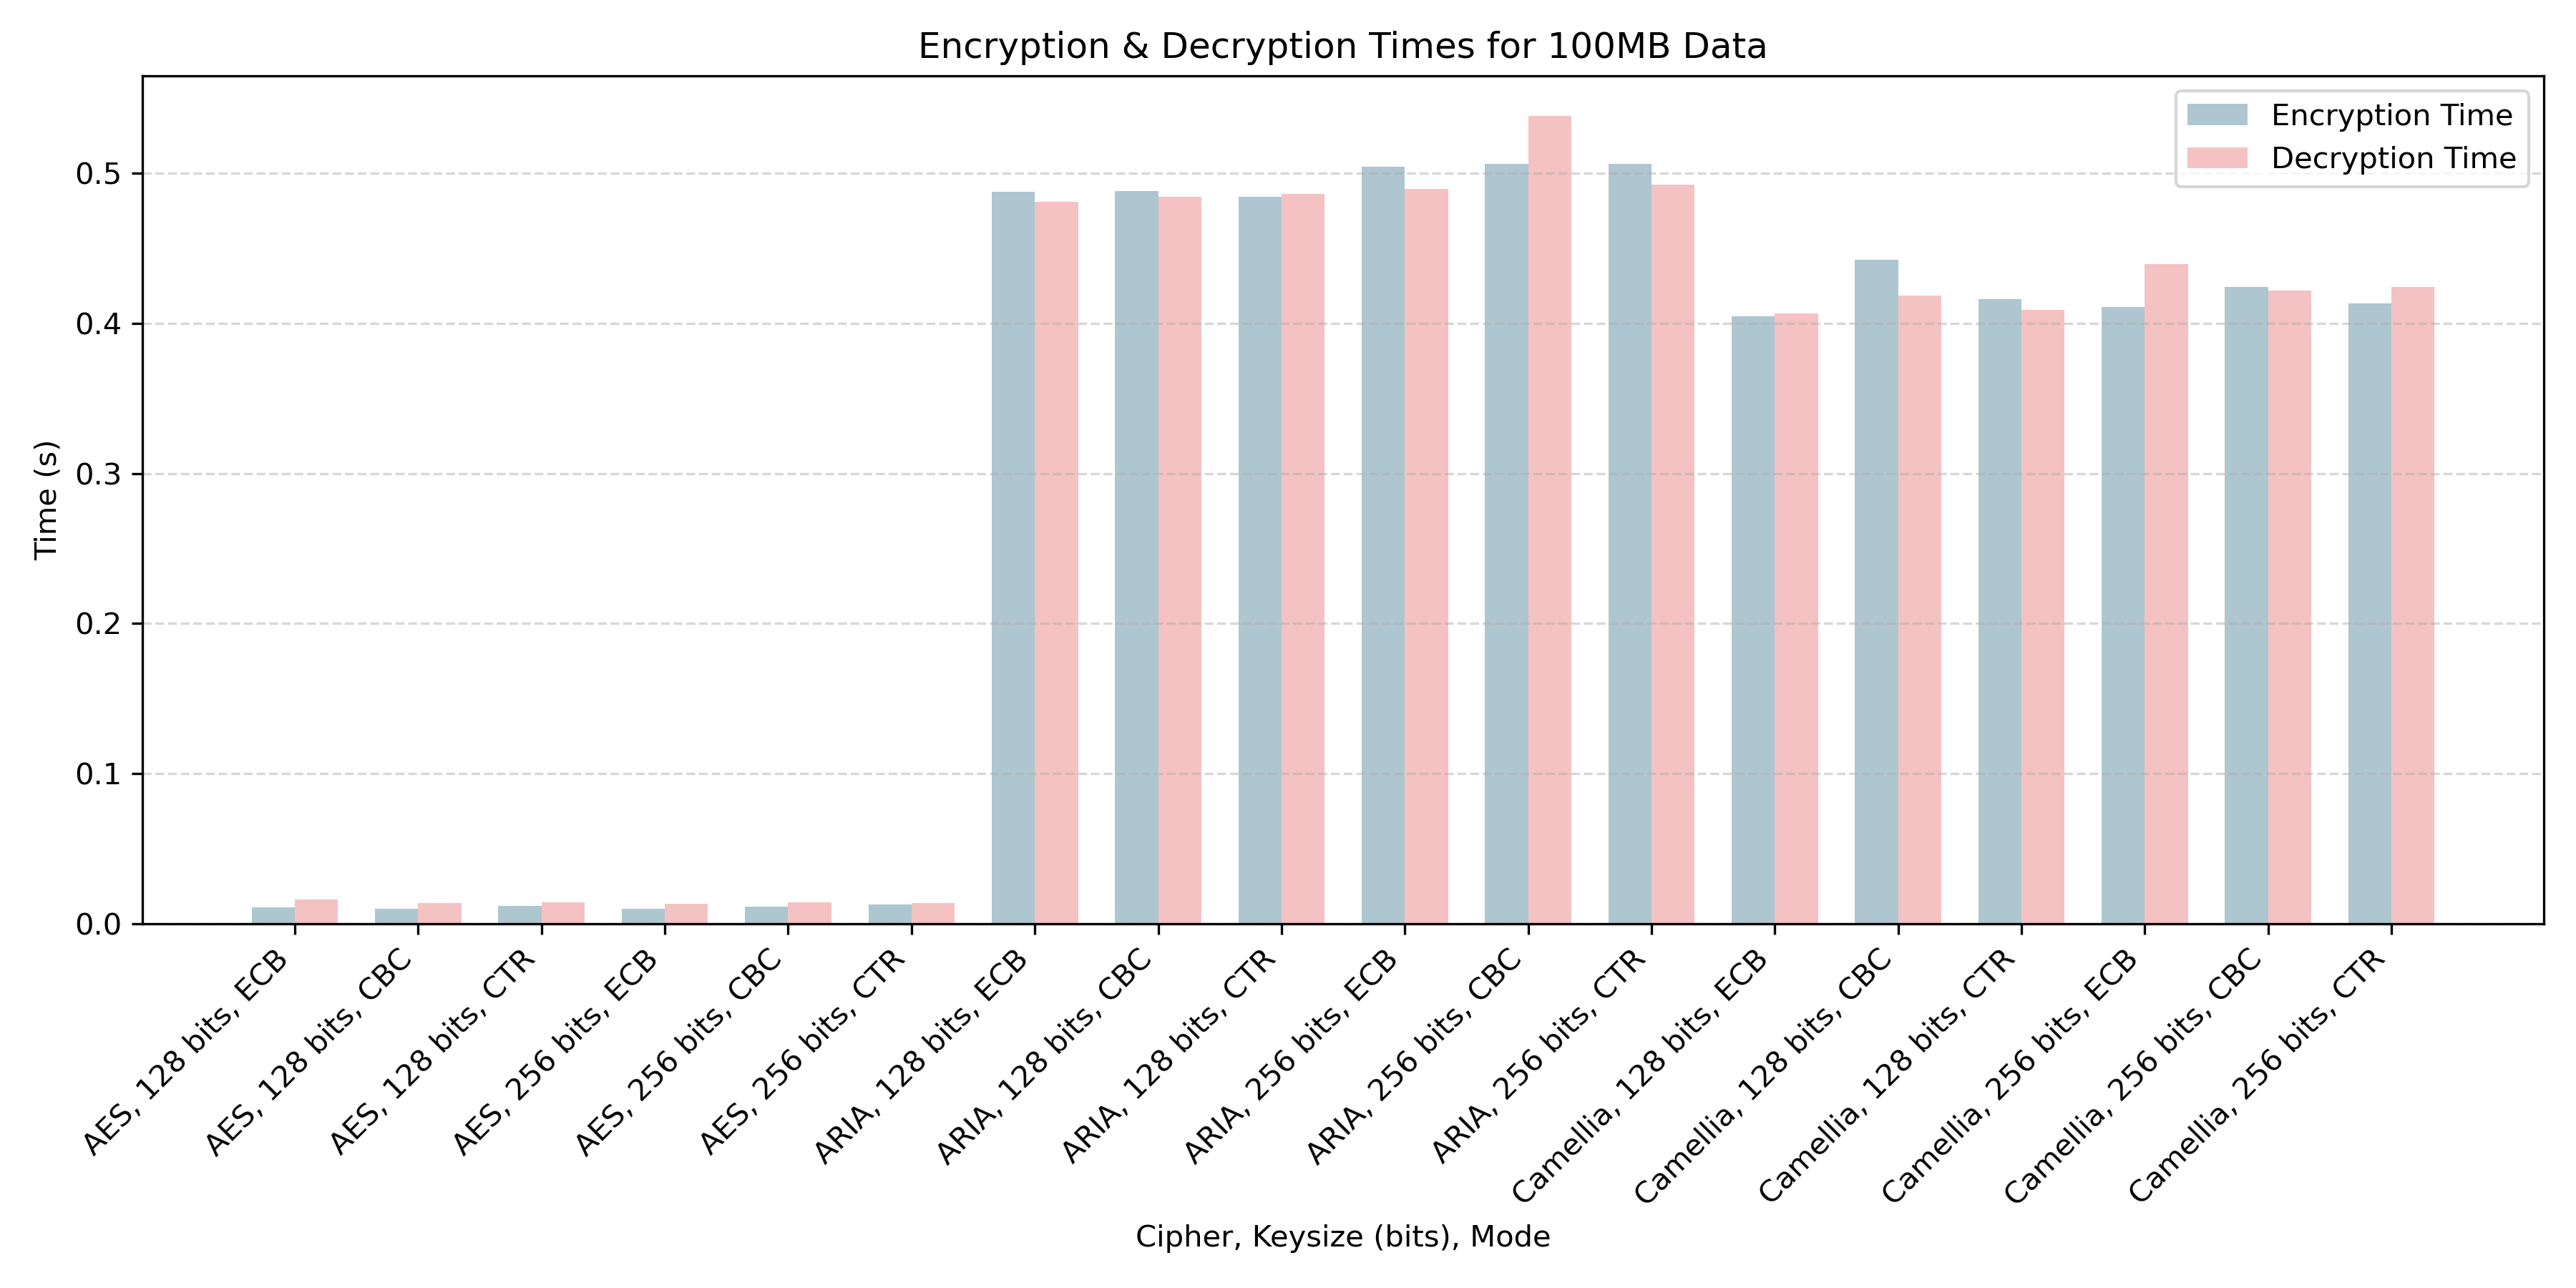
\includegraphics[width=\textwidth]{./images/100mb.png}
    \caption{Encryption \& decryption times for 100MB data}
\end{figure}

\begin{figure}[H]
    \centering
    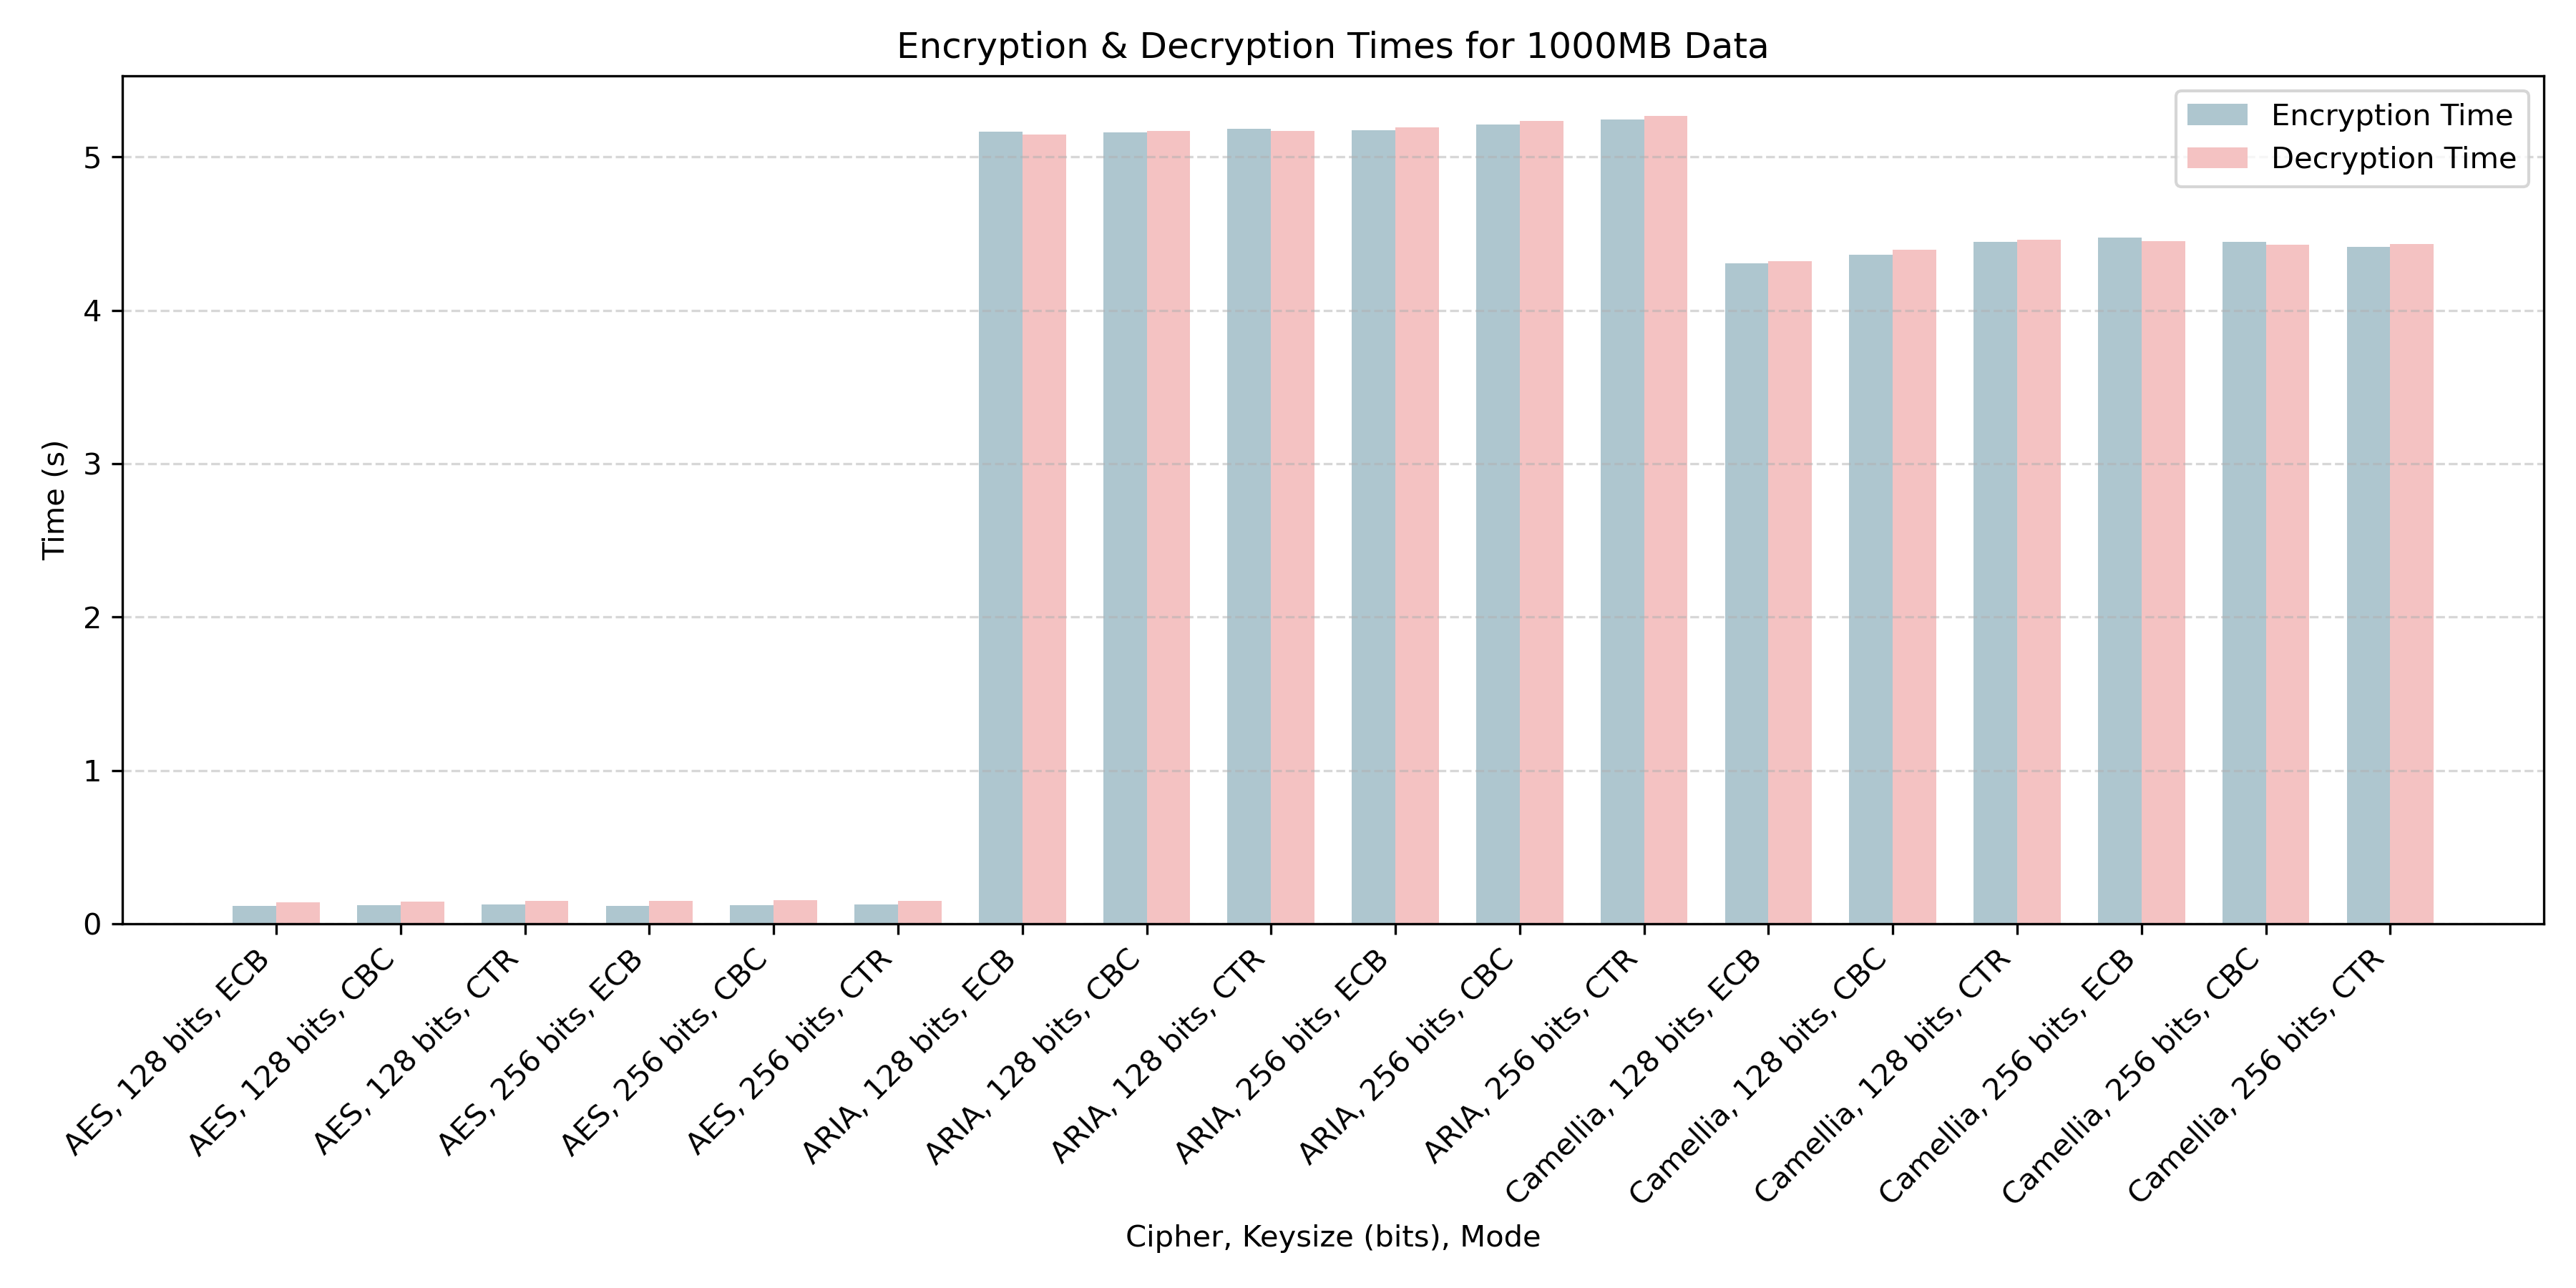
\includegraphics[width=\textwidth]{./images/1000mb.png}
    \caption{Encryption \& decryption times for 1000MB data}
\end{figure}


\section{Implementing \& Benchmarking Triple-DES}

\end{document}
